\documentclass{article}

\usepackage{microtype}
\usepackage{graphicx}
\usepackage{booktabs}
\usepackage{tabularx}
\usepackage{multirow}
\usepackage{float}
\usepackage{xurl}
\newcolumntype{L}{>{\raggedright\arraybackslash}X}
\usepackage{hyperref}
\newcommand{\theHalgorithm}{\arabic{algorithm}}
\usepackage{paperstyle}
\usepackage{amsmath}
\usepackage{amssymb}
\usepackage[capitalize,noabbrev]{cleveref}
\graphicspath{{../figures/}}
\hypersetup{pdftitle={Evaluating Agents as Served, Not as Weights}, pdfauthor={Haochuan Wang}}

% generated by paper/build.py - do not edit
\newif\ifjevresults
\jevresultsfalse
\newcommand{\jevscore}{}
\newcommand{\jevregret}{}
\newcommand{\jevlatency}{}
\newcommand{\jevdecisions}{}
\newcommand{\efivedecisions}{239}


\newcommand{\tsc}[1]{\texttt{#1}}
\icmltitlerunning{Evaluating Agents as Served, Not as Weights}

\begin{document}

\twocolumn[
  \icmltitle{Evaluating Agents as Served, Not as Weights}
  \begin{icmlauthorlist}
    \icmlauthor{Haochuan Wang}{mit}
  \end{icmlauthorlist}
  \icmlaffiliation{mit}{Massachusetts Institute of Technology, Cambridge, MA, USA}
  \icmlcorrespondingauthor{Haochuan Wang}{hcw@mit.edu}
  \icmlkeywords{agents, LLM serving, decision models, evaluation, Tetris}
  \vskip 0.3in
]

\printAffiliationsAndNotice{}

\begin{abstract}
An agent meets a model as served: through an endpoint with a price card, a shared cache and other tenants, or on whatever hardware a self-hosted model runs. Benchmarks rank the weights. We measure what agents get from models as served, using Tetris as an exact instrument: every move is scored against an oracle and every agent receives the same pieces. In five pre-specified experiments with about 20,000 calls to nine open-weight models on one serverless provider, plus an open decision model self-hosted on a CPU, we find that price and size do not predict decision quality; that resending history costs almost nothing when cached input is free, would cost eleven to twelve times more if it were not, and makes play worse; that deployments keep between 4 and more than 64 agent contexts warm, in line with their throughput rather than the model's KV-cache size; that an agent's own long requests slow its slowest short decisions more than tenfold, which a simple admission rule cuts by 59\% without hurting play; and that the decision model plays mid-pack but takes 27\,s per move on a CPU, about 650 times longer than reported on a GPU. Architecture predicts some of what an agent sees; the deployment sets the rest.
\end{abstract}

\begin{figure*}[t]
  \centering
  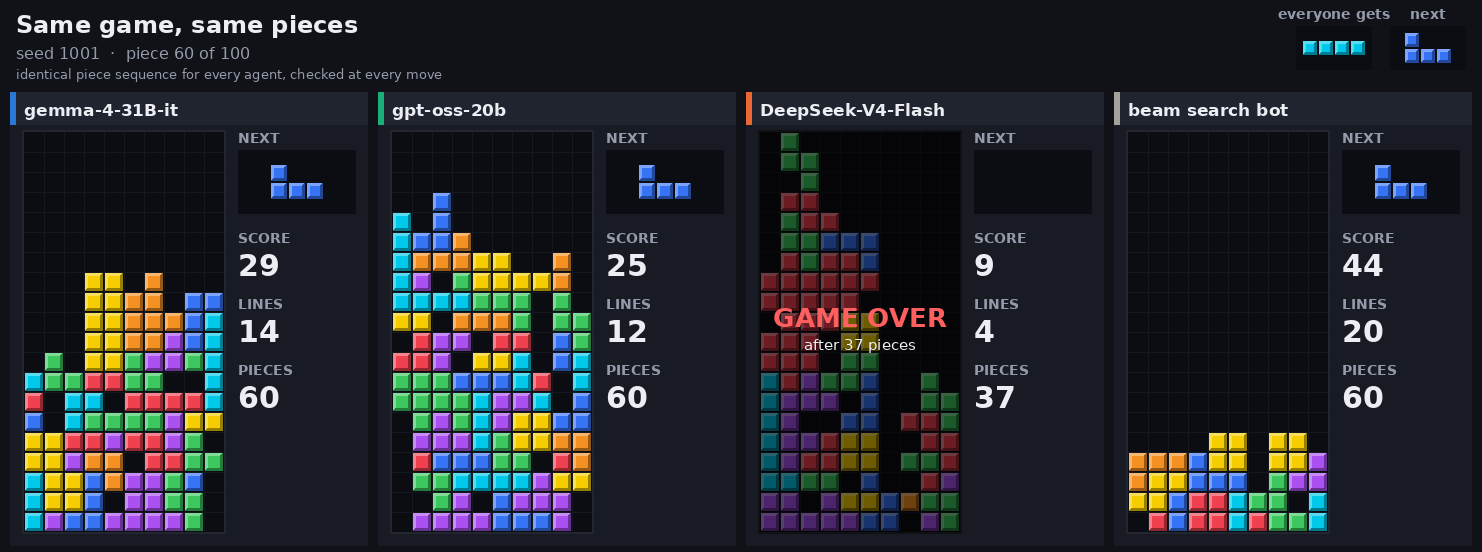
\includegraphics[width=0.92\textwidth]{teaser.png}
  \caption{\textbf{Same game, same pieces, five agents} (seed 1002, piece 60 of 100). Three open-weight language models served by Tensormesh and the Intelif decision model self-hosted on a CPU, replayed move by move from their logs, next to a beam-search bot. gpt-oss-20b and DeepSeek-V4-Flash have topped out; Intelif's stack is high, but it finishes all 100 pieces with 54 points, behind gemma-4-31B (76). Animations for more games are in the repository's \tsc{gallery/}.}
  \label{fig:teaser}
\end{figure*}

\section{Introduction}

An agent built on a language model rarely runs the model itself. It calls an endpoint, and behind the endpoint sit an inference engine, a cache, a scheduler and a price list, all shared with other tenants. The agent adds its own habits: how much history it resends, how many requests it keeps in flight, and whether long and short requests share a queue. What the agent receives, a decision of some quality at some latency and price, comes from all of these together.

Evaluations mostly rank the weights. Agent and game benchmarks report task quality through an API and treat serving as fixed; serving systems are evaluated on servers their authors control, with quality held constant. For open-weight models the gap is sharpest: one checkpoint can be served by many providers, quantized, cached and priced differently. A newer kind of model widens it. Decision models such as TypeSafe's Jev and the open Intelif do not generate text; they score a caller's options in one forward pass \citep{jev,intelif}. Their appeal is speed, and speed is a property of where a model runs.

We measure what agents get from models as served, from the only place an agent stands: the client side. Tetris is the instrument \citep{algorta}. Every move can be scored against an oracle, every game replays exactly, and every agent can be given the same pieces (\cref{fig:teaser}). We made about 20,000 calls to nine open-weight models on one serverless provider, Tensormesh, and self-hosted Intelif on a 4-core CPU. Four findings stand out:
\begin{itemize}\setlength\itemsep{1pt}
  \item \textbf{Price and size do not buy decisions.} The most expensive model played worst; the best play came from a 117B model at \$0.015 per 100 moves.
  \item \textbf{Deployments keep 4 to more than 64 concurrent agent contexts warm.} The number follows the deployment's throughput, not the model's KV-cache size.
  \item \textbf{An agent's own long requests slow its short ones.} The 95th-percentile time to a move grows from 1\,s to 11\,s; deferring the long requests cuts it by 59\% at the same cost, on held-out data.
  \item \textbf{A decision model is fast only where it is served.} Intelif played fifth of ten agents on the same games, always legally, but took 27\,s per move on our CPU against about 40\,ms reported on one GPU.
\end{itemize}
Our contributions are a measurement design that separates what an agent controls, observes and cannot see (\cref{sec:setup}); five pre-specified experiments that link deployment properties to cost, latency and decision quality, read against each model's published architecture (\cref{sec:models,sec:method,sec:results}); and an open, replayable harness that logs every call and plays the same games against hosted or self-hosted decision models.

\section{What an Agent Can See}
\label{sec:setup}

\Cref{tab:setup} lists the layers between a Tetris agent and the weights, what our agent varies at each layer, what it can observe, and what stays hidden. For the served models we vary only the top two layers and the choice of model. Everything we say about the engine is inferred from timing and reported token counts, so we state it as a hypothesis consistent with the data, not as a measurement.

\begin{table*}[t]
\caption{The measurement setup, layer by layer. E1--E4 call Tensormesh's serverless API (vLLM with LMCache); E5 runs a decision model in our own container. Engine internals are never observed directly.}
\label{tab:setup}
\centering\small
\begin{tabularx}{\textwidth}{@{}>{\raggedright\arraybackslash}p{2.6cm}LLL@{}}
\toprule
Layer & What the agent varies (experiment) & What it observes & What stays hidden \\
\midrule
Task: Tetris & nothing: every agent gets the same seeded pieces & board, current and next piece, legal placements; oracle regret per move & nothing (fully observed) \\
Agent harness & model (E1), history resent (E2), concurrent agents (E3), request mix and admission (E4) & its own queue and timing & nothing \\
Serverless API & output limits, JSON schema, priority hints (E4) & latency; reported prompt, cached and output tokens; refusals (HTTP 429); the public price card & billing records, routing, replica count, other tenants \\
Inference engine & nothing & only indirectly: cache hits, prefill throughput & batching, scheduler, KV memory pool, eviction and offloading \\
Weights & which served model id (E1--E4) & model card and config: parameters, attention and KV design & the exact checkpoint and quantization behind an id \\
Decision model & hardware, numeric precision, threads (E5) & the probability of every option; exact compute time & self-hosted: nothing; hosted Jev: its deployment \\
\bottomrule
\end{tabularx}
\end{table*}

\section{Related Work}

\textbf{Serving systems.} Continuous batching \citep{orca}, paged KV memory in vLLM \citep{vllm}, chunked prefill \citep{sarathi} and prefill/decode disaggregation \citep{distserve,splitwise} make engines fast; KV reuse across requests is handled by RadixAttention \citep{sglang}, multi-turn caching \citep{cachedattn}, KV-centric designs \citep{mooncake} and cache layers such as LMCache \citep{lmcache}. Agent-aware engines schedule whole programs \citep{autellix}. This work assumes control of the server; we ask what of it reaches a tenant. Client-side scheduling for black-box APIs has been studied in simulation \citep{yuan}; we test its simplest form on a live endpoint, with open-loop load \citep{schroeder} and tail metrics \citep{tail}.

\textbf{Benchmarks and audits.} AgentBench \citep{agentbench}, BALROG \citep{balrog} and lmgame-Bench \citep{lmgame}, which includes Tetris, score decisions through an API; HELM \citep{helm} adds efficiency metrics, and MLPerf Inference \citep{mlperf} measures serving stacks at fixed accuracy. Audits show that deployments differ: prompt caches shared across users \citep{gu}, undetectable model substitution \citep{cai}, and vendor differences for one open model \citep{k2}. We measure what such differences cost an agent.

\textbf{Decision models.} TypeSafe calls models that return calibrated probabilities over a caller's options, rather than text, ``System One'' models. Its Jev is hosted only, in early access, and is described by its makers as ``neither small nor an LLM'', with end-to-end responses of 70--500\,ms \citep{typesafe,jev}; TypeSafe does not publish results on public benchmarks. Intelif accepts the same request format: Qwen3-4B \citep{qwen3} with a LoRA adapter \citep{lora} and a linear scorer that reads one anchor token per option, so a single forward pass scores every option \citep{intelif}. Its authors report 31.77 on the third-party Decision Index \citep{dindex} at a median of 16.5\,ms on one RTX PRO 6000 GPU, and about 40\,ms per Tetris move. \ifjevresults We test both: Intelif where an agent without a GPU would run it, and Jev through TypeSafe's API.\else We test Intelif where an agent without a GPU would run it; Jev requires an early-access key, and we release a runner that plays the same games against it (\cref{app:decision}).\fi

\section{Models, and What Their Architecture Predicts}
\label{sec:models}

The provider serves nine open-weight models (\cref{tab:models}). If the weights alone decided what an agent experiences, two published quantities should matter most. The first is the KV cache one agent context occupies, which bounds how many contexts a given memory can keep; across these models it differs by a factor of 64. The second is the number of active parameters, which sets the compute to read a prompt, about two FLOPs per active parameter per token plus attention; it differs by a factor of 11.

\begin{table*}[t]
\caption{The models. Parameters and attention design are from each model's report, card or config. KV/ctx is our estimate of the 16-bit KV cache (plus the fixed recurrent state of Gated DeltaNet layers) that one 5.5k-token agent context needs, computed from the published config; real engines may store less (e.g., FP8). Prices are the provider's list prices per million input and output tokens; the provider states that cached input is free on every model. $^a$Active parameters from the MiniMax-M2 card (same architecture). $^b$Not on the price page, which lists the previous version (Qwen3.6-27B, Kimi K2.6, GLM-5.1) at these prices.}
\label{tab:models}
\centering\footnotesize
\begin{tabularx}{\textwidth}{@{}lrLrrl@{}}
\toprule
Model & Total / active & Attention and KV design & KV/ctx & \$/M in, out & Source \\
\midrule
gpt-oss-20b & 21B / 3.6B & alternating full and 128-token window; GQA, 8 KV heads & 132 MB & 0.07, 0.28 & \citet{gptoss} \\
gpt-oss-120b & 117B / 5.1B & same pattern, 36 layers & 198 MB & 0.15, 0.60 & \citet{gptoss} \\
gemma-4-31B & 31B dense & 5 sliding (1,024) : 1 global; keys reused as values & 1,015 MB & 0.14, 0.56 & \citet{gemma4} \\
DeepSeek-V4-Flash & 284B / 13B & compressed sparse (4$\times$) and compressed (128$\times$) attention; FP8 cache & 21 MB & 0.14, 0.28 & \citet{dsv4} \\
MiniMax-M2.5 & 229B / 10B$^a$ & full attention in all 62 layers; GQA, 8 KV heads & 1,335 MB & 0.30, 1.20 & \citet{minimax} \\
Qwen3.5-397B & 397B / 17B & 3 Gated DeltaNet : 1 full attention, 60 layers & 342 MB & 0.60, 3.60 & \citet{qwen35} \\
Qwen3.8-27B & 27B dense & 3 Gated DeltaNet : 1 full attention, 64 layers & 489 MB & 0.32, 3.20$^b$ & model card \\
Kimi-K2.7 & 1T / 32B & latent attention (512 + 64); INT4 experts & 370 MB & 0.96, 4.00$^b$ & \citet{kimi} \\
GLM-5.2 (NVFP4) & 744B / 40B & latent + DeepSeek sparse attention, shared indexer & 525 MB & 1.40, 4.40$^b$ & \citet{glm5} \\
\midrule
Intelif (self-hosted) & 4.0B dense & Qwen3-4B, full attention, GQA; LoRA + scorer & 775 MB & -- & \citet{intelif} \\
Jev (hosted) & not disclosed & ``neither small nor an LLM'' & -- & 0.042, free & \citet{typesafe} \\
\bottomrule
\end{tabularx}
\end{table*}

The models shrink the KV cache in different ways. Grouped-query attention shares key--value heads across query heads \citep{gqa}; sliding-window layers keep only the last 128 (gpt-oss) or 1,024 (gemma) tokens; latent attention stores one compressed vector per token, which cut the KV cache by 93\% in DeepSeek-V2 \citep{dsv2}; DeepSeek-V4 compresses further and keeps an FP8 cache. Sparse attention reduces attention compute rather than memory, although its indexer still scales quadratically \citep{dsv32,indexcache}. The Qwen models replace three of every four attention layers with Gated DeltaNet \citep{gdn}, a recurrent layer with a fixed-size state. Such hybrids are harder to prefix-cache: vLLM stores their state only at block boundaries, a mode it marks experimental \citep{vllmhybrid}. MiniMax kept full attention in every layer, citing high cache-hit rates in real conversations as one reason \citep{minimax}. These designs give three predictions an agent can check from outside: if memory per context limited caching, capacity should fall as KV per context grows (P1); cold prefill time should grow with active parameters (P2); and the hybrid models should report only part of a repeated prefix as cached (P3).

\section{Method}
\label{sec:method}

\textbf{Task.} The board is $10\times20$ with one piece of preview, and pieces are drawn uniformly at random from a generator seeded per game. The piece sequence depends only on the seed, never on how much an agent simulates, so all agents face identical games. Games stop at 100 pieces or when the stack tops out.

\textbf{Language-model agents (E1--E4).} Each move, the agent receives the board, the current and next piece, and the legal placements, each annotated with its simulated outcome (lines cleared, resulting height and holes). It answers with a JSON object naming one placement; in E1 and E2 a JSON schema restricts the output to legal placements. gpt-oss models run at low reasoning effort (gpt-oss-120b also at medium, as a separate configuration); gemma, Qwen, GLM and Kimi have thinking switched off through their chat template, and DeepSeek-V4-Flash answers directly by default. MiniMax-M2.5 cannot disable reasoning and exceeded 2,048 reasoning tokens on every move in a smoke test, so it appears only in E3.

\textbf{Decision-model agents (E5).} A decision model receives the same board and pieces; each legal placement is one option, described in words by its simulated outcome, following Intelif's own Tetris example, and the agent plays the most probable option. Intelif runs on the container we used for everything else: a 4-core Intel Xeon at 2.8\,GHz with AVX-512 and no GPU. We keep the released bf16 weights but compute in fp32, which on three test positions picked the same moves as bf16 with probabilities within 0.003, three times faster; dynamic int8 was seven times faster but changed the first move, so we did not use it.\ifjevresults{} Jev receives the identical request at TypeSafe's endpoint, pinned to \tsc{jev-1.13.0}.\fi

\textbf{Outcomes.} Quality is the game score relative to a beam-search bot on the same seeds, pooled over seeds as $(\sum \text{score} - \sum \text{random}) / (\sum \text{beam} - \sum \text{random})$, and the per-move regret against an approximate oracle that scores every legal placement by rollouts and a narrow beam search with common random numbers. Latency is wall time per decision measured by the client. Cost is estimated from list prices and the token counts the API reports. The provider states that cached input is free on every model, but four model cards show no cached price and billing records cannot be read with an inference key, so we report cost under the stated policy and, where it matters, an upper bound that bills cached input at the full input price.

\textbf{Capacity probe (E3).} $N$ agents each send a unique context of about 5.5k tokens (a random nonce in the system prompt followed by eight turns of a game) with a one-token output, stay idle for 30\,s, then send the same context plus one turn. An agent counts as warm when the second request reports at least half of the first one's prompt as cached and both requests succeeded. GLM-5.2 reports no cached tokens, so its hits are inferred from latency (second request faster than 0.35 of its cold median); this rule agrees with reported hits on 92\% of agents on the eight models that report them. $N$ runs from 1 to 64 in randomized order, with one to five repetitions per model depending on price. Aggregate prefill throughput is $N$ times the context length divided by the slowest first request of the round.

\textbf{Design and statistics.} Hypotheses, metrics and decision rules for every experiment were written down before its data; \cref{app:experiments} lists every deviation. Games are the independent unit: intervals for scores and paired differences come from 2,000 bootstrap resamples of seeds, and rank correlations are bootstrapped the same way. Hit rates carry Wilson 95\% intervals. E4 uses a two-level paired bootstrap over time blocks and requests. To keep our own traffic from contaminating cache and latency measurements, E3 ran alone, E1 and E2 ran together, and E4 ran alone; E5 sends no traffic to the provider. Every call is logged raw (timestamps, status, reported tokens, response text and, for decision models, the probability of every option), and every figure is regenerated from these logs.

\section{Results}
\label{sec:results}

\subsection{Price and size do not buy decisions (E1)}

\Cref{fig:ladder} places nine configurations by price, size and how well they play, over ten seeds and 6,403 decisions. The best play came from gpt-oss-120b, which reached 0.59 of the beam-search bot's score at low reasoning effort for \$0.015 per 100 decisions and 1.5\,s per move; medium effort reached 0.60 at six times the price and eight times the latency. gemma-4-31B followed at 0.52 for \$0.011. The most expensive model, GLM-5.2 at \$0.156 per 100 decisions, played worst (0.09), and the largest, Qwen3.5-397B, reached 0.23. Across the nine configurations the rank correlation between score and price was $-0.17$ (95\% bootstrap interval $-0.40$ to $-0.07$), with total parameters $-0.33$ ($-0.59$ to $-0.05$) and with active parameters $-0.41$ ($-0.63$ to $-0.23$), meeting our pre-specified criterion that neither price nor size shows a positive association. Per-move oracle regret orders the configurations almost identically, from 0.49 for gpt-oss-120b to 2.9 for GLM-5.2. A smaller, three-seed run of the same configurations ordered them quite differently (gemma 0.88, Kimi 0.85), a reminder that game benchmarks with few seeds rank noisily.

\begin{figure*}[t]
  \centering
  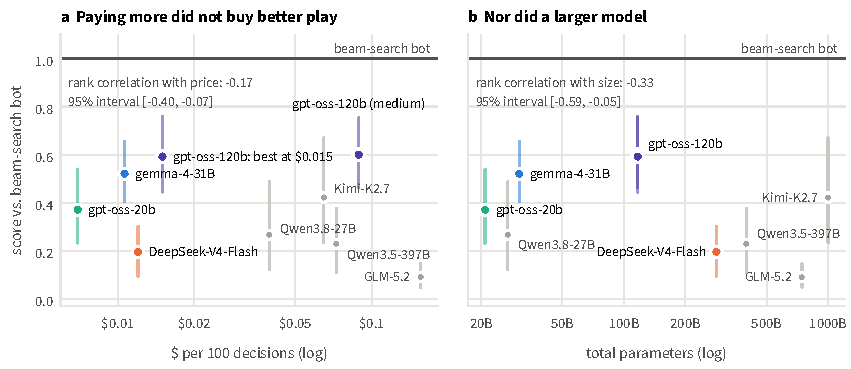
\includegraphics[width=\textwidth]{ladder.pdf}
  \caption{\textbf{Neither price nor size predicts how well a model plays.} Score relative to a beam-search bot on the same seeds (pooled over ten seeds; bars: 95\% bootstrap intervals over seeds) against the estimated price per 100 decisions (a) and total parameters (b), nine configurations served by Tensormesh, no history, output constrained to legal placements. The four models used throughout the paper are colored; the others are gray.}
  \label{fig:ladder}
\end{figure*}

\subsection{What history costs, and what it does to play (E2)}

Agents carry memory by resending history. We compared three policies on four models: no history, appending every turn, and keeping the last eight turns (\cref{fig:memory}). Appending lets the cache do its job: the prompt grows past 10k tokens, yet 90--97\% of it is served from cache, so the tokens actually processed per move stay at 500--740 on three models, about the same as with no history (620--830). The eight-turn window is the expensive choice: dropping the oldest turn rewrites the prefix right after the system prompt, so every move re-processes 4.4k--5.2k tokens, 5.7 to 10 times as many as appending (paired over seeds; 95\% intervals within about 10\%). Qwen3.8 shows the hybrid cost of \cref{sec:capacity} in a real game: appending leaves about 1,475 tokens per move uncached, twice the other models, and its 1.15k-token prompt without history is never cached at all, because it is shorter than one cache block.

\begin{figure*}[t]
  \centering
  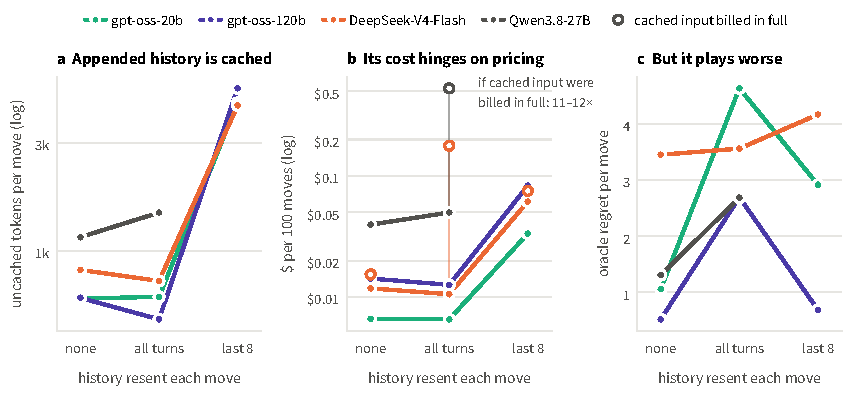
\includegraphics[width=\textwidth]{memory.pdf}
  \caption{\textbf{Appending history is cheap only because the cache absorbs it, and it plays worse.} Three history policies on four models, 6--7 paired seeds each. (a) Prompt tokens per move not served from cache. (b) Estimated cost under the provider's stated pricing (cached input free); hollow markers show the cost if cached input were billed at the full input price, which matters for the two models whose cards list no cached price. (c) Oracle regret per move. 4,168 calls.}
  \label{fig:memory}
\end{figure*}

Who pays for the cache decides whether appending is cheap. Under the provider's stated policy, appending costs 0.89 to 1.27 times as much as no history on every model. If cached input were billed at the full price, as two of the four model cards would literally suggest, appending would cost 11 times as much on DeepSeek-V4-Flash (95\% CI 9.5--12.6) and 12 times on Qwen3.8 (8.9--15.2), while staying at 0.9--1.0 on the gpt-oss models. Quality points the other way. The board is fully visible, so history adds no information, and appending lowered every model's score relative to the bot: gpt-oss-20b from 0.40 to 0.03, gpt-oss-120b from 0.60 to 0.24, Qwen3.8 from 0.39 to 0.13 and DeepSeek from 0.20 to 0.11. Per-move regret rose by 3.6 on gpt-oss-20b (95\% CI 2.9--4.3, seven paired seeds) and by 2.2 on gpt-oss-120b (1.9--2.7); on Qwen3.8 ($+1.6$, $-0.5$ to $3.5$) and on DeepSeek, which already played poorly without history ($+0.03$, $-1.1$ to $1.4$), the change was not distinguishable from zero. The memory that is cheapest to serve is the one that plays worst, consistent with evidence that long, repetitive context degrades the use of its relevant part \citep{lost}.

\subsection{How many agents a deployment keeps warm (E3)}
\label{sec:capacity}

Every deployment cached a repeated 5.5k-token context when one agent used it. How many agents it could serve that way differed by more than an order of magnitude (\cref{fig:capacity}; all nine models in \cref{fig:capacityall}). gpt-oss-20b and gpt-oss-120b kept all 64 concurrent contexts warm after 30\,s of idleness, the most we tested. MiniMax-M2.5 kept 32 and Qwen3.5-397B all 32 it was tested with; gemma-4-31B, Qwen3.8-27B and Kimi-K2.7 kept 16; GLM-5.2 kept 8; DeepSeek-V4-Flash kept 4. Beyond capacity the loss is abrupt: gemma kept 98\% of 16 contexts but 2\% of 32, and an evicted context took 12 to 19 times longer to serve again (2.3\,s instead of 0.19\,s on gemma; 6.3\,s instead of 0.33\,s on DeepSeek). Past capacity most deployments also refused requests: at 32 or 64 agents, 62\% of DeepSeek's agents and 54\% of gemma's had a request refused with HTTP 429, while the gpt-oss deployments refused none.

\begin{figure*}[t]
  \centering
  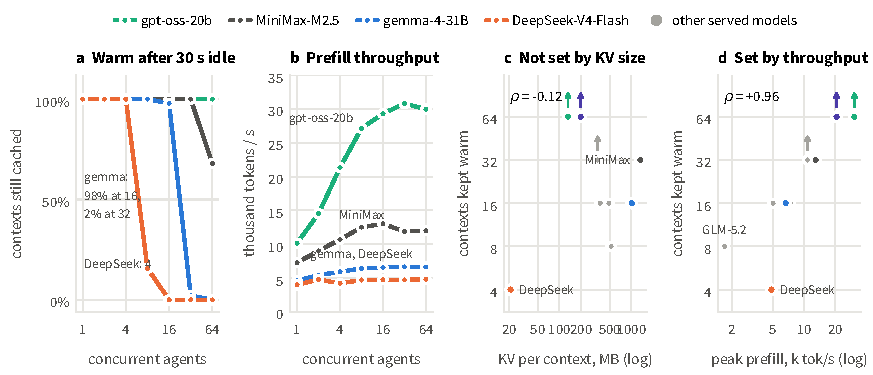
\includegraphics[width=\textwidth]{capacity.pdf}
  \caption{\textbf{How many agent contexts a deployment keeps warm follows its throughput, not the model's KV-cache size.} $N$ agents each send a unique 5.5k-token context, wait 30\,s and send it again. (a) Share still served from cache and (b) aggregate prefill throughput, for the four models whose curves show the pattern most clearly (all nine in \cref{fig:capacityall}). (c, d) Capacity, the largest $N$ with at least 90\% of contexts still cached, against the KV cache one context needs and against the deployment's peak aggregate prefill throughput; arrows mark capacities at the largest $N$ tested; $\rho$ is Spearman's rank correlation over nine models. 5,542 calls.}
  \label{fig:capacity}
\end{figure*}

The architecture does not explain the ranking (P1). The model with the smallest KV cache per context, DeepSeek-V4-Flash at an estimated 21\,MB, keeps the fewest contexts, and the one with the largest, MiniMax-M2.5 at 1.3\,GB, keeps 32; across the nine models the rank correlation between capacity and KV size is $-0.12$. What capacity does track is how much prefill work a deployment can do at once ($\rho = +0.96$). gpt-oss-20b's aggregate throughput grew from 10k to 31k tokens per second as agents were added, a sign of many parallel replicas, while DeepSeek stayed near 4.8k and gemma near 6.6k, as if requests were processed by a single replica in turn. Measured in tokens, DeepSeek's capacity also matches a smaller run two days earlier with 15k-token contexts: it kept one context but not four then (between 15k and 60k tokens), and four 5.5k contexts but not eight now (between 22k and 44k). Even 44k tokens of DeepSeek's compact cache is about 150\,MB by our estimate, far below the KV memory of one GPU, so the limit is a property of how much cache and hardware the deployment allots, or of how many other tenants share it, not of the model.

Two architectural predictions do hold. Cold prefill took longer on models with more active parameters (P2; Spearman $+0.82$ across the nine models), from 0.54\,s on gpt-oss-20b to 1.5\,s on Kimi and 3.6\,s on GLM-5.2. And the two Gated DeltaNet hybrids reported only part of a repeated prefix as cached (P3): Qwen3.5 always 5,280 of 5,684 tokens (93\%) and Qwen3.8 always 4,704 (83\%), exactly the prompt rounded down to a multiple of a large block, as block-aligned caching of the recurrent state predicts. The other models cache all but at most the last 140 tokens. A Qwen3.8 agent therefore re-pays up to about 1.5k tokens of prefill on every turn.

\begin{figure}[!t]
  \centering
  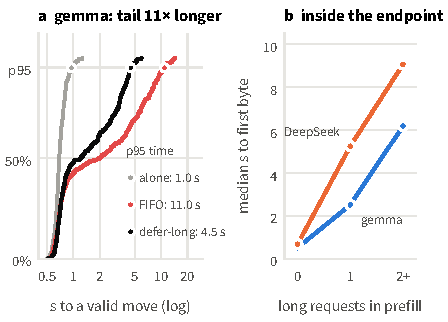
\includegraphics[width=\columnwidth]{interference.pdf}
  \caption{\textbf{Long requests stretch the tail of short decisions, inside the endpoint.} Short (about 1k-token) decisions sent alone or mixed with long (about 19k-token) requests at identical arrival times, ten time blocks per model. (a) Time from scheduled arrival to a valid move on gemma-4-31B, with each policy's 95th percentile. (b) Endpoint time to first byte of a short request under FIFO, by the number of long requests still waiting for their own first byte when it was sent.}
  \label{fig:interference}
\end{figure}

\begin{figure*}[t]
  \centering
  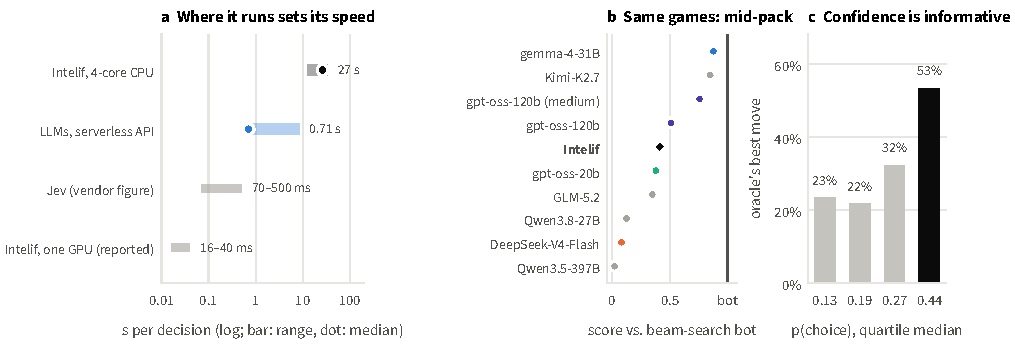
\includegraphics[width=\textwidth]{decision.pdf}
  \caption{\textbf{A decision model is fast only where it is served.} (a) Seconds per decision: Intelif on our 4-core CPU (30 positions re-timed on an otherwise idle machine) and the nine language-model configurations through the serverless API (their median latencies), against the figures reported for Intelif on one GPU and by TypeSafe for Jev (gray). (b) Score relative to the beam-search bot on the same three games (seeds 1000--1002) for the decision model(s) and the nine language-model configurations. (c) How often Intelif chose the oracle's best move, by quartile of the probability it gave its choice (60 moves per quartile).}
  \label{fig:decision}
\end{figure*}

\subsection{An agent's own long requests slow its short ones (E4)}

Agents mix traffic: short per-move decisions and, now and then, long requests that summarize or plan over a large context. We replayed the same frozen requests, at the same arrival times, under four client policies: short requests alone, everything in one first-in-first-out (FIFO) queue, the same queue with vLLM-style priority hints, and defer-long, which sends a long request only when no short one is waiting or in flight, keeps at most one long request outstanding, and stops deferring after 6\,s. The requests come from a held-out corpus that no earlier run touched, with ten time blocks per model and hypotheses and margins fixed in advance.

Mixing in long requests raised the 95th-percentile time to a valid move from 0.95\,s to 11.0\,s on gemma-4-31B ($+1{,}052\%$, 95\% CI $+689\%$ to $+1{,}386\%$) and from 1.8\,s to 22.4\,s on DeepSeek-V4-Flash ($+1{,}123\%$, CI $+372\%$ to unbounded), confirming the first hypothesis on both (\cref{fig:interference}). Most of the delay arises inside the endpoint, not in our queue: a short request's median time to first byte grew from 0.5\,s to 2.5\,s with one long request still in prefill and to 6.2\,s with two on gemma (0.7, 5.3 and 9.1\,s on DeepSeek), while a plain network probe moved by less than 0.2\,s. Priority hints, which the endpoint accepts, changed nothing measurable (gemma $-2\%$, CI $-16\%$ to $+5\%$). Defer-long cut gemma's tail by 59\% (CI 45\% to 66\%) and raised the rate of useful decisions by 24\% at the same cost, passing every pre-specified non-inferiority check, including the per-move regret margin. On DeepSeek, defer-long cut the tail by 46\% and raised useful decisions by 23\%, but about 4\% of short decisions never produced a valid move under mixed load, so the tail interval is unbounded and that hypothesis remains inconclusive. Defer-long cannot help short requests that arrive while a long one is already in prefill, and it makes long requests wait longer.

\subsection{Decision models as served (E5)}

Intelif answered every move with a legal placement and a probability for each option, so no output had to be parsed, retried or replaced. Over three games and 239 moves it reached 0.41 of the beam-search bot's score, fifth of the ten agents that played these seeds, between gpt-oss-120b at low effort (0.51) and gpt-oss-20b (0.38), although Tetris is not among its training tasks (\cref{fig:decision}b). Its per-move regret, 1.28, fell between the stronger language models (0.38--0.85) and the weaker ones (2.1--3.7). Its speed is where serving matters most. On the container's four CPU cores each move took a median of 26.5\,s, re-timed on 30 positions with nothing else running (31\,s during play, when other jobs shared the cores), growing linearly with the prompt at about 28\,ms per input token. Its authors report about 40\,ms per Tetris move and a median of 16.5\,ms on their benchmark, both on one GPU, roughly 650 times faster than our CPU with the same weights, while the language models answered in a median of 0.6--0.7\,s through the serverless API (\cref{fig:decision}a). Its probabilities carry information at the top end: on the quarter of moves where it gave its choice more than 0.34, regret was 0.30 and it picked the oracle's best move 53\% of the time, against 22--32\% in the other quarters (\cref{fig:decision}c), so an agent could use them to decide when to fall back to search or a larger model.
\ifjevresults
Jev, called through TypeSafe's public API, played the same three games: it reached \jevscore{} of the bot's score with a per-move regret of \jevregret{}, at a median of \jevlatency{} per move including the network round trip, over \jevdecisions{} moves.
\fi

\section{Discussion}

\textbf{What the weights predict, and what they do not.} Published architecture predicted two things an agent can see from outside: how long a cold prompt takes (active parameters) and how much of a repeated prompt a hybrid model can reuse (block-aligned caching of its recurrent state). It did not predict the outcome that matters most for an agent fleet, how many agents a deployment keeps warm, which followed the hardware behind the deployment rather than the compactness of the model's KV cache. Neither did price or size predict how well a model played: the most expensive model played worst, and gpt-oss-120b at low reasoning effort matched its own medium-effort play at a sixth of the price. A leaderboard row reports none of this.

\textbf{What to report.} An evaluation of an agent on a served model should state the provider and model identifier, the date, the full price card including cached input and how it was applied, the cache behavior the API reports (granularity and hit rate at the agent's concurrency), refusals under load, the agent's memory and admission policy, and, for self-hosted models, the hardware and numeric precision. Each factor we varied or measured changed an outcome here by a factor of two or more. Measuring them is inexpensive: the four API experiments cost \$9.27 under the provider's stated pricing (\$13.55 at the full-price upper bound).

\textbf{Decision models.} A decision model removes generation, parsing and invalid outputs from the loop: Intelif always returned a legal move, with probabilities informative enough to decide when to escalate. Its selling point, speed, belongs to the hardware: on the CPU an agent without a GPU would use, it was about 40 times slower than a far larger language model behind a serverless API. Comparisons between decision models and language models should state where each one ran.

\section{Limitations}

All API measurements come from one provider over two days, on a shared platform whose other traffic we cannot see; they describe these deployments at that time, not the models in general. Model identifiers do not prove which checkpoint or quantization was served. Capacity is measured with one context length, one idle gap and one to five repetitions per model, and refusals at high load also reduce the number of contexts that reached the cache. Costs are estimates from list prices and reported token counts. The oracle is approximate. Tetris has a fully visible state, which is likely why history did not help; tasks with hidden state may reward memory. The decision-model comparison covers three games with the prompt format of Intelif's own example; other prompts or hardware may change it. E2 and E4 used fewer calls than planned because of the budget (\cref{app:experiments}).

\section{Conclusion}

For an agent, the product is not the weights but the model as served: behind a price card and a cache, next to other tenants, on whatever hardware runs it, and driven by the agent's own habits. Measured from the client, these factors changed what the agent paid by up to an order of magnitude, its tail latency by more than an order of magnitude, how many agents could share a deployment by a factor of sixteen, and a decision model's speed by roughly 650 times; price and size did not predict how well an agent played. Published architecture explained part of this, the deployment the rest. Evaluations of open-weight and decision models should report the serving context alongside the score.

\bibliography{references}
\bibliographystyle{paperstyle}

\newpage
\appendix
\onecolumn
\raggedbottom

\section{Experiments, Calls and Deviations}
\label{app:experiments}

\begin{table}[H]
\caption{The five experiments. Calls are model calls, including failures (E3: mostly HTTP 429 refusals at high load). Cost is estimated from list prices and reported tokens, under the provider's stated pricing (cached input free) and under the full-price bound that our budget guard used; the guard's ledger also reserves cost for failed calls. The whole study, including the smaller earlier runs cited in the text, stayed within \$20 by the guard's accounting.}
\label{tab:experiments}
\centering\small
\begin{tabularx}{\textwidth}{@{}lLrrr@{}}
\toprule
Experiment & Design & Calls & \$ stated & \$ bound \\
\midrule
E1 model ladder & 9 configurations $\times$ 10 seeds $\times$ $\leq$100 pieces; no history, annotated, schema-constrained & 6,403 & 3.02 & 3.04 \\
E2 history policy & 4 models $\times$ 3 policies (Qwen3.8: 2) $\times$ 9 seeds; 73 of 99 games finished & 4,168 & 1.31 & 3.62 \\
E3 cache capacity & 9 models $\times$ $N \in \{1, \dots, 64\}$ $\times$ 1--5 repetitions & 5,542 & 3.63 & 5.58 \\
E4 interference & 2 models $\times$ 10 time blocks $\times$ 4 conditions; held-out corpus & 3,630 & 1.31 & 1.31 \\
E5 decision models & Intelif on a 4-core CPU, 3 games (seeds 1000--1002)\ifjevresults; Jev, same games\fi & \efivedecisions & 0 & 0 \\
\bottomrule
\end{tabularx}
\end{table}

\textbf{Deviations from the written plans.} All are recorded with timestamps in the repository (\tsc{notes/scaleup\_plan.md}). (i) The first part of E3 was stopped after rounds with 32 or more agents of different models overlapped and drew gateway-wide refusals; later parts never overlapped such rounds, and 17 rounds in flight during an overlap are excluded. The second part stopped at its budget cap and a third ran the five remaining rounds. (ii) E2 dropped one arm (Qwen3.8 with the last eight turns) before any data to save budget, then reached its cap: 26 of 99 games did not finish and are excluded; paired contrasts use the 6--7 seeds on which every policy finished. (iii) Score relative to the beam-search bot is pooled over seeds rather than averaged per seed, decided after one E2 seed on which the bot itself scored 10 points made per-seed ratios explode, and before E1 and E5 were analyzed. (iv) E4 ran 10 time blocks per model instead of 13, set by a rule fixed before it ran (the largest number whose estimated cost fit the remaining budget). (v) E5 was reduced to three games for lack of CPU time; its process was once killed by the container's memory limit, and the interrupted game was replayed from the start, reproducing the first 22 moves with identical probabilities. (vi) The E1 and E2 oracle was computed after the API phase, with identical settings.

\section{Cache Capacity of Every Model}
\label{app:capacity}

\begin{figure}[H]
  \centering
  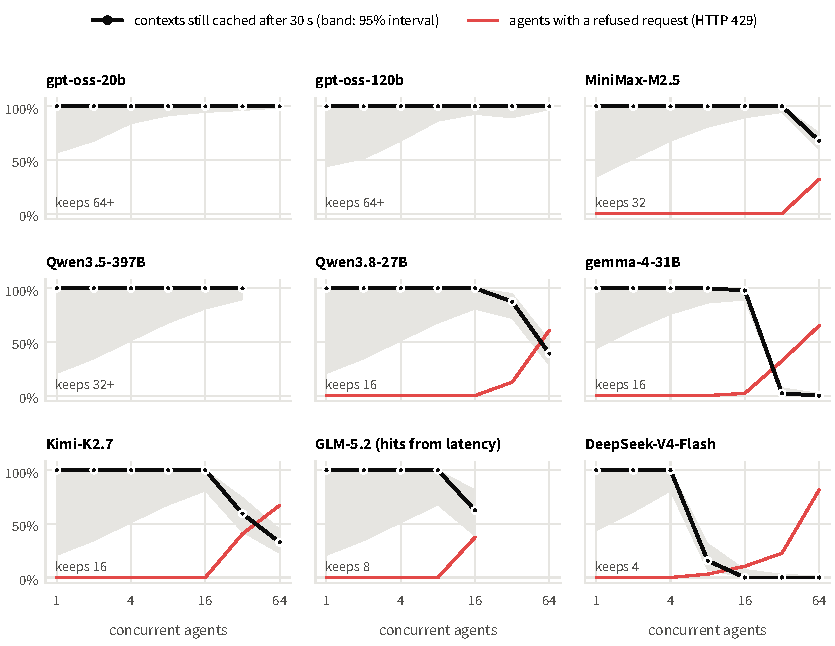
\includegraphics[width=0.75\textwidth]{capacity_all.pdf}
  \caption{Cache capacity of every served model, ordered by capacity. Each panel shows the share of agents whose context was still served from cache after 30\,s (line; band: Wilson 95\% interval over agents) and the share of agents with a refused request (red), against $N$ concurrent agents with 5.5k-token contexts. Rounds per point: 1--5 depending on the model's price. GLM-5.2 reports no cached tokens; its hits are inferred from latency, a rule that agrees with reported hits on 92\% of agents on the eight models that report them. Kimi-K2.7, Qwen3.8, Qwen3.5 and GLM-5.2 were measured with one repetition each, so their intervals are wide.}
  \label{fig:capacityall}
\end{figure}

\section{The Decision-Model Agents}
\label{app:decision}

\textbf{Request.} Each move is one Choice question in the \tsc{/v1/systemone} format that Intelif shares with Jev. The state holds the board as 20 rows of \tsc{\#} and \tsc{.}, the current piece and the next piece. Each legal placement is one option, keyed by rotation and column and described by its simulated outcome, following Intelif's own Tetris example, for instance ``rotation 0, column 3: clears no lines, no new holes, raises the stack by 2, surface gets bumpier''. The instruction reads ``You are playing Tetris. Where should the T piece land? Clear lines, avoid holes and keep the stack low and flat.'' Positions had 5 to 34 options and 290 to 1,220 input tokens. The language-model agents received the same facts as numbers, so \cref{fig:decision} compares agents as each is meant to be used, not the two kinds of model under identical inputs.

\textbf{Precision and determinism.} The container's CPU (Intel Xeon, 2.8\,GHz, AVX-512 with int8 dot products, no native bf16) runs the released bf16 weights slowly. Keeping the bf16 weights and computing in fp32 reproduced the bf16 choices on three test positions (probabilities within 0.003) at a third of the time. Dynamic int8 quantization was seven times faster but chose a different first move and spread probability over more options, so we did not use it. Play is deterministic: a replayed game reproduced its first 22 moves with identical probabilities.

\textbf{Hosted Jev.} The same runner plays against TypeSafe's hosted Jev: it sends the identical request with the model pinned to \tsc{jev-1.13.0}, retries rate-limited calls, records Jev's \emph{confidence} separately from its option probabilities (TypeSafe documents that the two differ), and never logs the API key. It needs no GPU and runs from a laptop, a small virtual machine or the provided Docker image (\tsc{deploy/jev/}); three games are about 240 calls and 0.2M input tokens. \ifjevresults The results above come from this runner.\else Running it requires an early-access key from TypeSafe.\fi

\section{Reproducing the Paper}

Every number and figure is regenerated from the committed raw logs (\tsc{calls.jsonl}, \tsc{rows.jsonl}, \tsc{requests.jsonl} and console logs in each run directory). Live experiments need provider API keys and stay within the budgets in \cref{tab:experiments}; everything else runs offline on a CPU. The repository's \tsc{README.md} lists the commands; \tsc{python paper/build.py} rebuilds every figure and this document, and \tsc{python scripts/build\_gallery.py} rebuilds every animation.

\end{document}
